%
% funktionen.tex
%
% (c) 2018 Prof Dr Andreas Müller
%
\section{Funktionenrämue
\label{section:funktionenraume}}
\rhead{Funktionräume}

\subsection{Vektorräume von Funktionen}

\subsection{Translation und Dilatation}
Der Definitionsbereich $\mathbb R$ zeichnet sich durch die darin zur
Verfügung stehenden Rechenoperationen aus.
Man kann zu einem Argument einen konstanten Wert hinzuaddieren oder mit
einer Zahl multiplizieren, bevor man eine Funktion auswertet.
Daraus ergeben sich die zwei Operationen der Translation und der Dilatation.

\begin{definition}
Sei $f$ eine Funktion auf $\mathbb R$ mit Werten in $Y$.
Dann setzt man
\begin{align*}
T_bf&\colon \mathbb R \to Y: t\mapsto f(t-b)&&\text{Translation}
\\
D_af&\colon \mathbb R \to Y: t\mapsto f(t/a)&&\text{Dilatation}
\end{align*}
\end{definition}

% XXX TODO Graphik zur Visualisierung von T_b und D_a
\begin{figure}
\centering
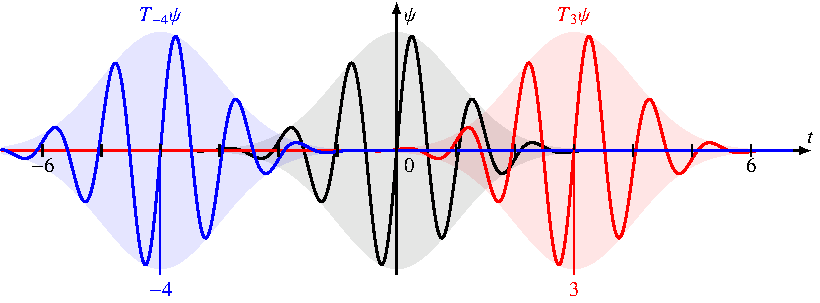
\includegraphics[width=\hsize]{chapters/1-geometrie/images/translation.pdf}
\caption{Wirkung des Operators $T_b$ auf das Gabor-Wavelet
$\psi(t) = e^{-t^2/2}\sin(6t)$,
der Graph von $T_b\psi$ ist um $b$ nach rechts verschoben.
\label{geometrie:Tb:image}}
\end{figure}
\begin{figure}
\centering
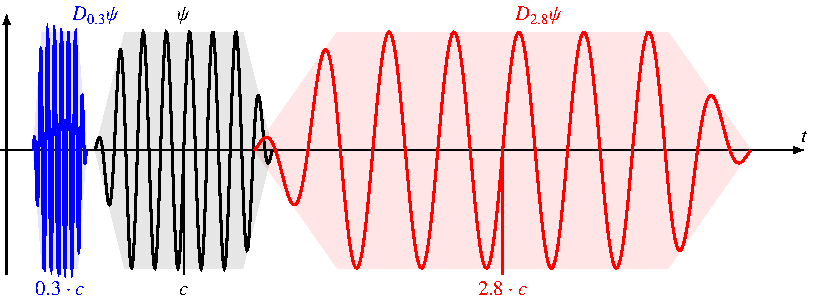
\includegraphics[width=\hsize]{chapters/1-geometrie/images/dilatation.pdf}
\caption{Wirkung des Operators $D_a$ auf ein im Punkt $c$ zentriertes
Wavelet $\psi$. Das Wavelet $D_a\psi$ ist zentriert im Punkt $a\cdot c$.
\label{geometrie:Da:image}}
\end{figure}


\begin{satz}
Translation $T_b$ und Dilatation $D_a$ sind lineare Abbildungen.
Die beiden Operatoren vertauschen nicht, vielmehr gilt
$T_bD_a = D_aT_{ab}$.
\end{satz}

\begin{proof}[Beweis]

Wir berechnen die Wirkung beider Operatoren in verschiedener Reihenfolge
nach:
\begin{align*}
(D_aT_bf)(t)
&=
(T_bf)(t/a)
=
f((t-b)/a) = f(t/a - b/a)
\\
(T_bD_a f)(t)
&=
(D_af)(t - b)
=
f(t/a - b)
=
f(((t-ab)/a)
\\
&=
(D_aT_{ab}f)(t)
\end{align*}
\end{proof}

% XXX TODO Graphik zur Illustration der Rechenregeln für T_b und D_a

\begin{satz}
Die einzigen stetigen Funktionen, die Eigenvektoren von $T_b$ sind für
jeden beliebigen Wert von $b$ sind die Funktionen $t\mapsto e^{i\omega t}$.
\end{satz}

\begin{proof}[Beweis]
Sei $f$ eine Eigenfunktion aller Operatoren $T_b$ mit Eigenwert $\lambda(b)$.
 kann keine Nullstelle haben.
Wäre nämlich $f(t_0)=0$, dann würde folgen
\[
(T_bf)(t_0) = f(t_0-b) = \lambda(b) f(t_0) = 0,
\]
die Funktion würde identisch verschwinden.

Weiter kann man aus der Stetigkeit von $f$ schliessen, dass auch
\[
\lambda(b) = \frac{f(t)}{f(t-b)}
\]
eine stetige Funktion von $b$ ist, die keine Nullstellen hat.
\end{proof}

Dieser Satz erklärt die besondere Stellung, die den komplexen
Exponentialfunktionen in der Fourier-Theorie zukommt.
